\RequirePackage{luatex85} % tuftebook not yet compatible with recent luatex

\documentclass[twoside,bahasa]{tufte-book}

%\usepackage[T1]{fontenc}
%\usepackage[utf8]{luainputenc}

\setlength{\parskip}{\smallskipamount}
\setlength{\parindent}{0pt}

\usepackage{fontspec}
\setmonofont{DejaVu Sans Mono}

\usepackage{amsmath}
\usepackage{amssymb}


\usepackage{minted}
\newminted{python}{breaklines,fontsize=\footnotesize}
\newminted{text}{breaklines,fontsize=\footnotesize}
\newcommand{\txtinline}[1]{\mintinline[fontsize=\footnotesize]{text}{#1}}
\newcommand{\pyinline}[1]{\mintinline[fontsize=\footnotesize]{python}{#1}}

% Using background color for minted environment
\usepackage{xcolor}
\usepackage{mdframed}

\definecolor{mintedbg}{rgb}{0.95,0.95,0.95}
\BeforeBeginEnvironment{minted}{
    \begin{mdframed}[backgroundcolor=mintedbg,%
        topline=false,bottomline=false,%
        leftline=false,rightline=false]
}
\AfterEndEnvironment{minted}{\end{mdframed}}

\usepackage{pgfplots}
\pgfplotsset{width=7cm,compat=1.8}
\usepackage{pgfplotstable}

\usepackage{babel}



\title{Judul Buku}
\author[Fadjar \& Mariya]{\noindent{Fadjar Fathurrahman} \\[3mm]
\noindent{Mariya Al Qibtiya Nasution} \\[3mm]}
\publisher{Self-Published}


\begin{document}
\maketitle

\frontmatter

\tableofcontents
\listoffigures
\listoftables

\mainmatter

\chapter{Bab 1}

\section{Sub1}

Contoh paragraf. Contoh paragraf. Contoh paragraf. Contoh paragraf.
Contoh paragraf. Contoh paragraf. Contoh paragraf. Contoh paragraf.
Contoh paragraf.

\begin{pythoncode}
def myfunc1(x,y):
    return (x + y) / (x - y)
\end{pythoncode}

Contoh paragraf. Contoh paragraf. Contoh paragraf. Contoh paragraf.
Contoh paragraf. Contoh paragraf. Contoh paragraf. Contoh paragraf.
Contoh paragraf.

\begin{fullwidth}
Paragraf \emph{full-width}. Paragraf \emph{full-width}. Paragraf \emph{full-width}.
Paragraf \emph{full-width}. Paragraf \emph{full-width}. Paragraf \emph{full-width}.
Paragraf \emph{full-width}. Paragraf \emph{full-width}. Paragraf \emph{full-width}.
Paragraf \emph{full-width}. Paragraf \emph{full-width}. Paragraf \emph{full-width}.
\end{fullwidth}


Persamaan:
\begin{equation}
G(x,x') = \frac{1}{x - x'}
\end{equation}


Implementasi:

\begin{fullwidth}
\begin{pythoncode}
a_very_very_very_very_long_expr = 1 + 2 + 3 + 4 + sin(x) + cos(x)
\end{pythoncode}
\end{fullwidth}

\section{Sub2}

Contoh paragraf. Contoh paragraf. Contoh paragraf.~Contoh paragraf.
Contoh paragraf. Contoh paragraf.~Contoh paragraf. Contoh paragraf.
Contoh paragraf.
\footnote{Catatan samping. Ini hanya untuk
intermezzo semata. Tapi bisa menambahkan persamaan juga:
\begin{equation}
\alpha + \beta = \frac{\zeta}{\Omega} \int_{-\inf}^{+\inf} G(x)\,\mathrm{d}x
\end{equation}
}


\section{Sub3}

Contoh paragraf. Contoh paragraf. Contoh paragraf. Contoh paragraf.
Contoh paragraf. Contoh paragraf. Contoh paragraf. Contoh paragraf.
Contoh paragraf.

Contoh paragraf. Contoh paragraf. Contoh paragraf. Contoh paragraf.
Contoh paragraf. Contoh paragraf. Contoh paragraf. Contoh paragraf.
Contoh paragraf.
Contoh paragraf. Contoh paragraf. Contoh paragraf. Contoh paragraf.
Contoh paragraf. Contoh paragraf. Contoh paragraf. Contoh paragraf.
Contoh paragraf.

Contoh paragraf. Contoh paragraf. Contoh paragraf. Contoh paragraf.
Contoh paragraf. Contoh paragraf. Contoh paragraf. Contoh paragraf.
Contoh paragraf.

Contoh paragraf. Contoh paragraf. Contoh paragraf. Contoh paragraf.
Contoh paragraf. Contoh paragraf. Contoh paragraf. Contoh paragraf.
Contoh paragraf.

Contoh gambar
\begin{figure}[h]
\begin{tikzpicture}{width=7cm,compat=1.8}
  \begin{axis}[xlabel=Cost,ylabel=Error]
  \addplot[color=red,mark=x] coordinates {
    (2,-2.8559703)
    (3,-3.5301677)
    (4,-4.3050655)
    (5,-5.1413136)
    (6,-6.0322865)
    (7,-6.9675052)
    (8,-7.9377747)
  };
  \end{axis}
\end{tikzpicture}
\caption{Contoh gambar dengan TikZ}
\end{figure}

Contoh paragraf. Contoh paragraf. Contoh paragraf. Contoh paragraf.
Contoh paragraf. Contoh paragraf. Contoh paragraf. Contoh paragraf.
Contoh paragraf.


Contoh gambar lagi:
\begin{figure}[h]
{\centering
\begin{tikzpicture}
\begin{axis}[]
  \newcommand\MU{0}
  \newcommand\SIGMA{1e-3}
  \addplot[
    red,
    domain=-3*\SIGMA:3*\SIGMA,
  samples=201,]
    {exp(-0.5*(x-\MU)^2/\SIGMA^2) / (\SIGMA*sqrt(2*pi))};
\end{axis}
\end{tikzpicture}
\par
}
\caption{Contoh gambar dengan TikZ}
\end{figure}


Contoh paragraf. Contoh paragraf. Contoh paragraf. Contoh paragraf.
Contoh paragraf. Contoh paragraf. Contoh paragraf. Contoh paragraf.
Contoh paragraf.

Contoh paragraf. Contoh paragraf. Contoh paragraf. Contoh paragraf.
Contoh paragraf. Contoh paragraf. Contoh paragraf. Contoh paragraf.
Contoh paragraf.
Contoh paragraf. Contoh paragraf. Contoh paragraf. Contoh paragraf.
Contoh paragraf. Contoh paragraf. Contoh paragraf. Contoh paragraf.
Contoh paragraf.

\begin{marginfigure}
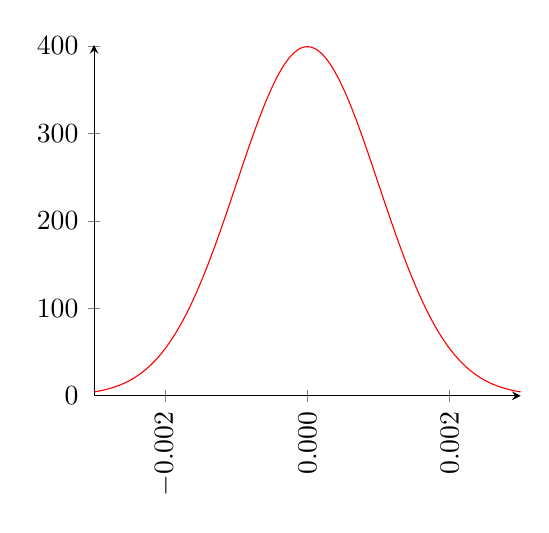
\begin{tikzpicture}
\begin{axis}[
  axis lines=left,
  scaled ticks=false,
  xticklabel style={
    rotate=90,
%    anchor=east,
    /pgf/number format/precision=3,
    /pgf/number format/fixed,
    /pgf/number format/fixed zerofill,
  },
  ymin=0,
  ymax=401,
]
  % define various constants
  \newcommand\MU{0}
  \newcommand\SIGMA{1e-3}

  \addplot[
    red,
    domain=-3*\SIGMA:3*\SIGMA,
    samples=201
  ]
  { exp(-0.5*(x-\MU)^2/\SIGMA^2)/(\SIGMA*sqrt(2*pi)) };
\end{axis}
\end{tikzpicture}
\caption{This is a margin figure.}
\label{fig:marginfig}
\end{marginfigure}

Contoh paragraf. Contoh paragraf. Contoh paragraf. Contoh paragraf.
Contoh paragraf. Contoh paragraf. Contoh paragraf. Contoh paragraf.
Contoh paragraf.

Contoh paragraf. Contoh paragraf. Contoh paragraf. Contoh paragraf.
Contoh paragraf. Contoh paragraf. Contoh paragraf. Contoh paragraf.
Contoh paragraf.

Contoh paragraf. Contoh paragraf. Contoh paragraf. Contoh paragraf.
Contoh paragraf. Contoh paragraf. Contoh paragraf. Contoh paragraf.
Contoh paragraf.

\section{Sub lagi}

Contoh paragraf. Contoh paragraf. Contoh paragraf. Contoh paragraf.
Contoh paragraf. Contoh paragraf. Contoh paragraf. Contoh paragraf.
Contoh paragraf.

\subsection{Sub sub lagi}

Contoh paragraf. Contoh paragraf. Contoh paragraf. Contoh paragraf.
Contoh paragraf. Contoh paragraf. Contoh paragraf. Contoh paragraf.
Contoh paragraf.


\section{Sub lagi}

Contoh paragraf. Contoh paragraf. Contoh paragraf. Contoh paragraf.
Contoh paragraf. Contoh paragraf. Contoh paragraf. Contoh paragraf.
Contoh paragraf.

\subsection{Sub sub lagi}

Contoh paragraf. Contoh paragraf. Contoh paragraf. Contoh paragraf.
Contoh paragraf. Contoh paragraf. Contoh paragraf. Contoh paragraf.
Contoh paragraf.


\section{Sub lagi}

Contoh paragraf. Contoh paragraf. Contoh paragraf. Contoh paragraf.
Contoh paragraf. Contoh paragraf. Contoh paragraf. Contoh paragraf.
Contoh paragraf.

\subsection{Sub sub lagi}

Contoh paragraf. Contoh paragraf. Contoh paragraf. Contoh paragraf.
Contoh paragraf. Contoh paragraf. Contoh paragraf. Contoh paragraf.
Contoh paragraf.

\section{Sub lagi}

Contoh paragraf. Contoh paragraf. Contoh paragraf. Contoh paragraf.
Contoh paragraf. Contoh paragraf. Contoh paragraf. Contoh paragraf.
Contoh paragraf.

\subsection{Sub sub lagi}

Contoh paragraf. Contoh paragraf. Contoh paragraf. Contoh paragraf.
Contoh paragraf. Contoh paragraf. Contoh paragraf. Contoh paragraf.
Contoh paragraf.

\section{Sub lagi}

Contoh paragraf. Contoh paragraf. Contoh paragraf. Contoh paragraf.
Contoh paragraf. Contoh paragraf. Contoh paragraf. Contoh paragraf.
Contoh paragraf.

\subsection{Sub sub lagi}

Contoh paragraf. Contoh paragraf. Contoh paragraf. Contoh paragraf.
Contoh paragraf. Contoh paragraf. Contoh paragraf. Contoh paragraf.
Contoh paragraf.

\section{Sub lagi}

Contoh paragraf. Contoh paragraf. Contoh paragraf. Contoh paragraf.
Contoh paragraf. Contoh paragraf. Contoh paragraf. Contoh paragraf.
Contoh paragraf.

\subsection{Sub sub lagi}

Contoh paragraf. Contoh paragraf. Contoh paragraf. Contoh paragraf.
Contoh paragraf. Contoh paragraf. Contoh paragraf. Contoh paragraf.
Contoh paragraf.

\section{Sub lagi dengan simbol: $\alpha + \beta$}

Contoh paragraf. Contoh paragraf. Contoh paragraf. Contoh paragraf.
Contoh paragraf. Contoh paragraf. Contoh paragraf. Contoh paragraf.
Contoh paragraf.

\subsection{Sub sub lagi}

Contoh paragraf. Contoh paragraf. Contoh paragraf. Contoh paragraf.
Contoh paragraf. Contoh paragraf. Contoh paragraf. Contoh paragraf.
Contoh paragraf.



\chapter{Bab 2}

Contoh paragraf. Contoh paragraf. Contoh paragraf. Contoh paragraf.
Contoh paragraf. Contoh paragraf. Contoh paragraf. Contoh paragraf.
Contoh paragraf.

\section{Sub 1}

Contoh paragraf. Contoh paragraf. Contoh paragraf. Contoh paragraf.
Contoh paragraf. Contoh paragraf. Contoh paragraf. Contoh paragraf.
Contoh paragraf.

\subsection{Subsub1}

Contoh paragraf. Contoh paragraf. Contoh paragraf. Contoh paragraf.
Contoh paragraf. Contoh paragraf. Contoh paragraf. Contoh paragraf.
Contoh paragraf.


\end{document}
